\section{Methodology}
\label{sec:methodology}

In this section, we present the methodology for architecture optimization (AO) and filter optimization (FO) as well as details about how benchmark images are preprocessed, how AO and FO are evaluated across the benchmarks, and how these methods are implemented.

\subsection{Architecture Optimization (AO)}
\label{sec:ao}

Our approach for AO builds upon the work of Pinto et al.~\cite{Pinto:2009} and Bergstra et al.~\cite{Bergstra:2013}, i.e., fundamental, feedforward convolutional operations are stacked by means of hyperparameter optimization, leading to effective yet simple convolutional networks that do not require expensive filter optimization and from which prediction is done by linear support vector machines (SVMs).

Operations in convolutional networks can be viewed as linear and non-linear transformations that, when stacked, extract high level representations of the input. Here we use a well-known set of operations called (i) \emph{convolution} with a bank of filters, (ii) rectified linear \emph{activation}, (iii) spatial \emph{pooling}, and (iv) \emph{local normalization}. Appendix~\ref{sec:convnet_ops} provides a detailed definition of these operations.

We denote as \emph{layer} the combination of these four operations in the order that they appear in the left panel of Fig.~\ref{fig:framework}. Local normalization is optional and its use is governed by an additional ``yes/no'' hyperparameter. In fact, there are other six hyperparameters, each of a particular operation, that have to be defined in order to instantiate a layer. They are presented in the lower part of the left panel in Fig.~\ref{fig:framework} and are in accordance to the definitions of Appendix~\ref{sec:convnet_ops}.

Considering one layer and possible values of each hyperparameter, there are over 3,000 possible layer architectures, and this number grows exponentially with the number of layers, which goes up to three in our case (Fig.~\ref{fig:framework} right panel). In addition, there are network-level hyperparameters, such as the size of the input image, that expand possibilities to a myriad potential architectures.
 
 % and emphasize the need to rapidly evaluate candidate architectures.

 % and that we are interested in learning deep representations extracted with the combination of up to three of such layers (Fig.~\ref{fig:framework} right panel), the importance of hyperparameter optimization in this context becomes clear. 

% Considering one layer and possible values of each hyperparameter, there are over 3,000 possible layer architectures. Given that this number grows exponentially with the number of layers and that we are interested in learning deep representations extracted with the combination of up to three of such layers (Fig.~\ref{fig:framework} right panel), the importance of hyperparameter optimization in this context becomes clear. In addition, there are network-level hyperparameters that expand possibilities even more, like the size of the input image, or the depth of the candidate network.


The overall set of possible hyperparameter values is called \emph{search space}, which in this case is discrete and contains variables that are only meaningful in combination with others. For example, hyperparameters of a given layer are just meaningful if the candidate architecture has actually that number of layers.
In spite of the intrinsic difficulty in optimizing architectures in this space, \emph{random search} has played and important role in problems of this type~\cite{Pinto:2009,Bergstra:2012} and it is the strategy of our choice due to its effectiveness and simplicity.

We can see in Fig.~\ref{fig:framework} that a three-layered network has a total of 25 hyperparameters, seven per layer and four at network level. They are all defined in Appendix~\ref{sec:convnet_ops} with the exception of \emph{input size}, which seeks to determine the best size of the image's greatest axis (rows or columns) while keeping its aspect ratio. Concretely, random search in this paper can be described as follows:

\begin{enumerate}
\item Randomly --- and uniformly, in our case --- sample values from the hyperparameter \emph{search space};
\item Extract features from real and fake training images with the candidate architecture;
\item Evaluate the architecture according to an \emph{optimization objective} based on linear SVM scores;
\item Repeat steps 1--3 until a \emph{termination criterion} is met;
\item Return the best found convolutional architecture.
\\
\end{enumerate}



\begin{figure}
\begin{center}
 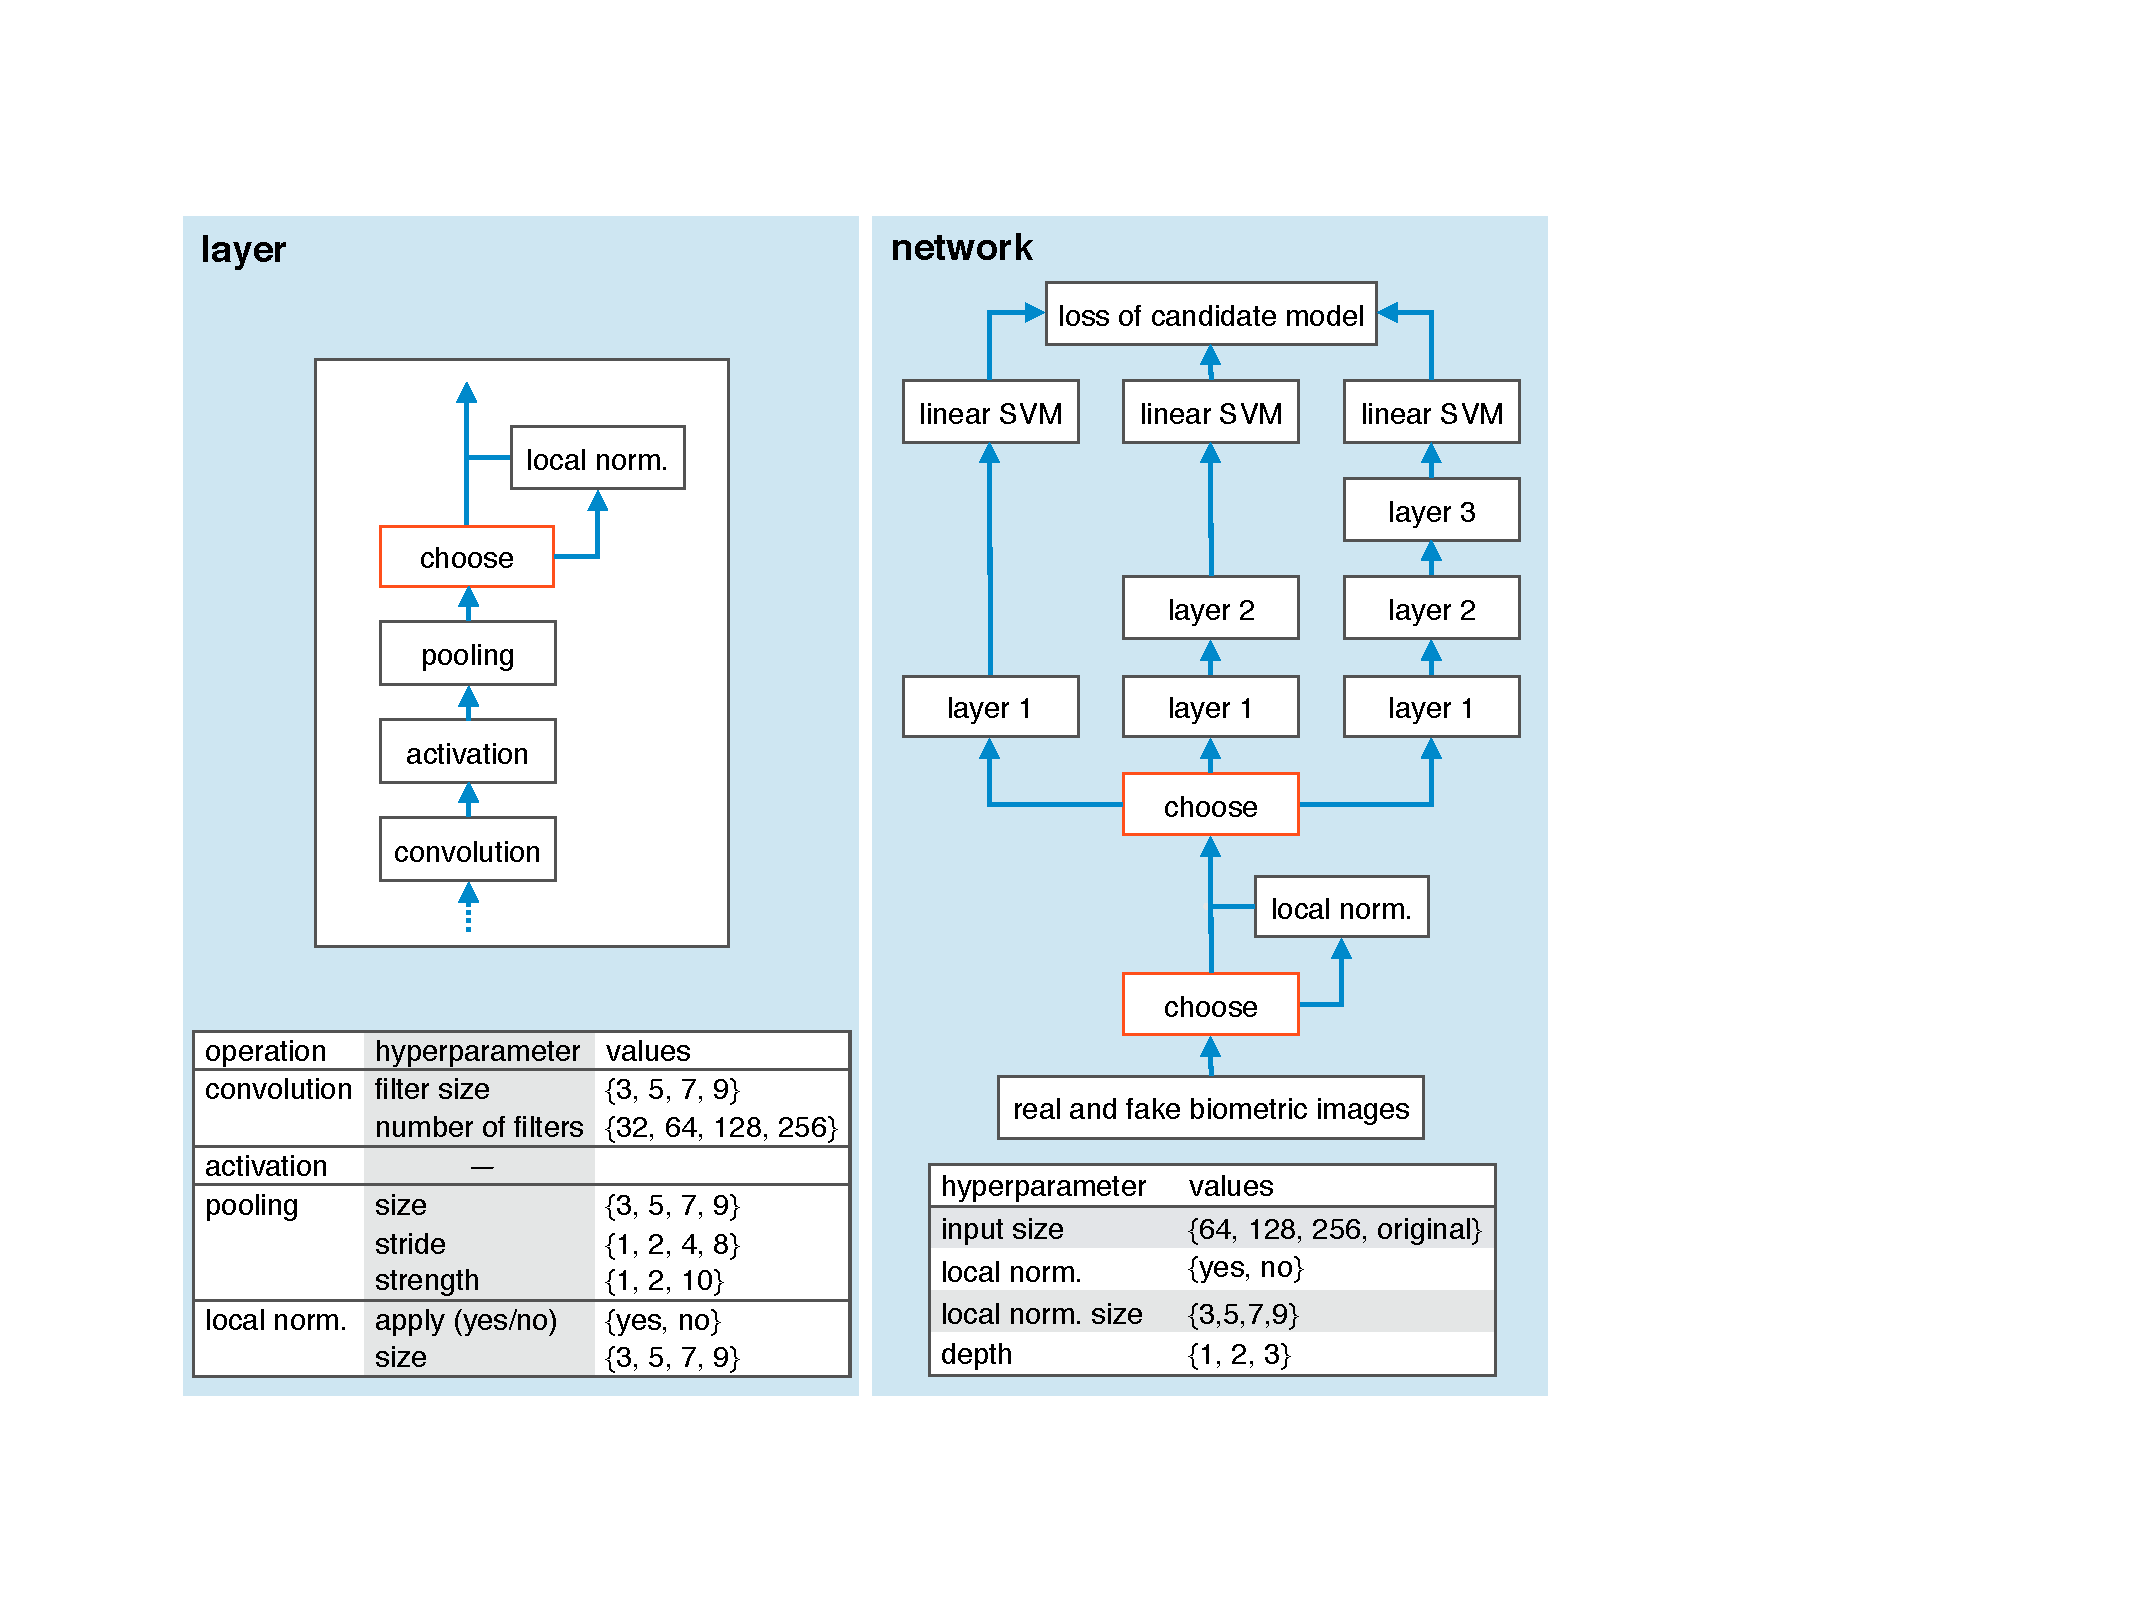
\includegraphics[width=1.0\linewidth]{hp-schema.pdf}
 \caption{Schematic diagram for architecture optimization (AO) illustrating how operations are stacked in a layer (left) and how the network is instantiated and evaluated according to possible hyperparameter values (right). Note that a three-layered convolutional network of this type has a total of 25 hyperparameters governing both its architecture and its overall behaviour through a particular instance of stacked operations.}
 \label{fig:framework}
\end{center}
\end{figure}


Even though there are billions of possible networks in the search space (Fig.~\ref{fig:framework}), it is important to remark that not all candidate networks are valid. For example, a large number of candidate architectures (i.e., points in the search space) would produce representations with spatial resolution smaller than one pixel. Hence, they are naturally unfeasible.
Additionally, in order to avoid very large representations, we discard in advance candidate architectures whose intermediate layers produce representations of over 600K elements or whose output representation has over 30K elements.

% Filter optimization is of paramount importance in convolutional networks and 

Filter weights are randomly generated for AO. This strategy has been successfully used in the vision literature~\cite{Pinto:2009,Saxe:2011,Pinto:2011b,Jarrett:2009} and is essential to make AO practical, avoiding the expensive filter optimization (FO) part in the evaluation of candidate architectures. We sample weights from a uniform distribution $U(0,1)$ and normalize the filters to zero mean and unit norm in order to ensure that they are spread over the unit sphere. When coupled with rectified linear activation (Appendix~\ref{sec:convnet_ops}), this sampling enforces sparsity in the network by discarding about $50$\% of the expected filter responses, thereby improving the overall robustness of the feature extraction.

A candidate architecture is evaluated by first extracting deep representations from real and fake images and later training hard-margin linear SVMs ($C$=$10^5$) on these representations.
We observed that the sensitivity of the performance measure was saturating with traditional 10-fold cross validation (CV) in some benchmarks. Therefore, we opted for a different validation strategy. Instead of training on nine folds and validating on one, we train on one fold and validate on nine. Precisely, the \emph{optimization objective} is the mean detection accuracy obtained from this adapted cross-validation scheme, which is maximized during the optimization.

For generating the 10 folds, we took special care in putting all samples of an individual in the same fold to enforce robustness to cross-individual spoofing detection in the optimized architectures.
Moreover, in benchmarks where we have more than one attack type (e.g., Replay-Attack and LivDet2013, see Section~\ref{sec:databases}), we evenly distributed samples of each attack type across all folds in order to enforce that candidate architectures are also robust to different types of attack.

Finally, the \emph{termination criterion} of our AO procedure simply consists of counting the number of valid candidate architectures and stopping the optimization when this number reaches 2,000.


\subsection{Filter Optimization (FO)}
\label{sec:fo}

\begin{figure}
\begin{center}
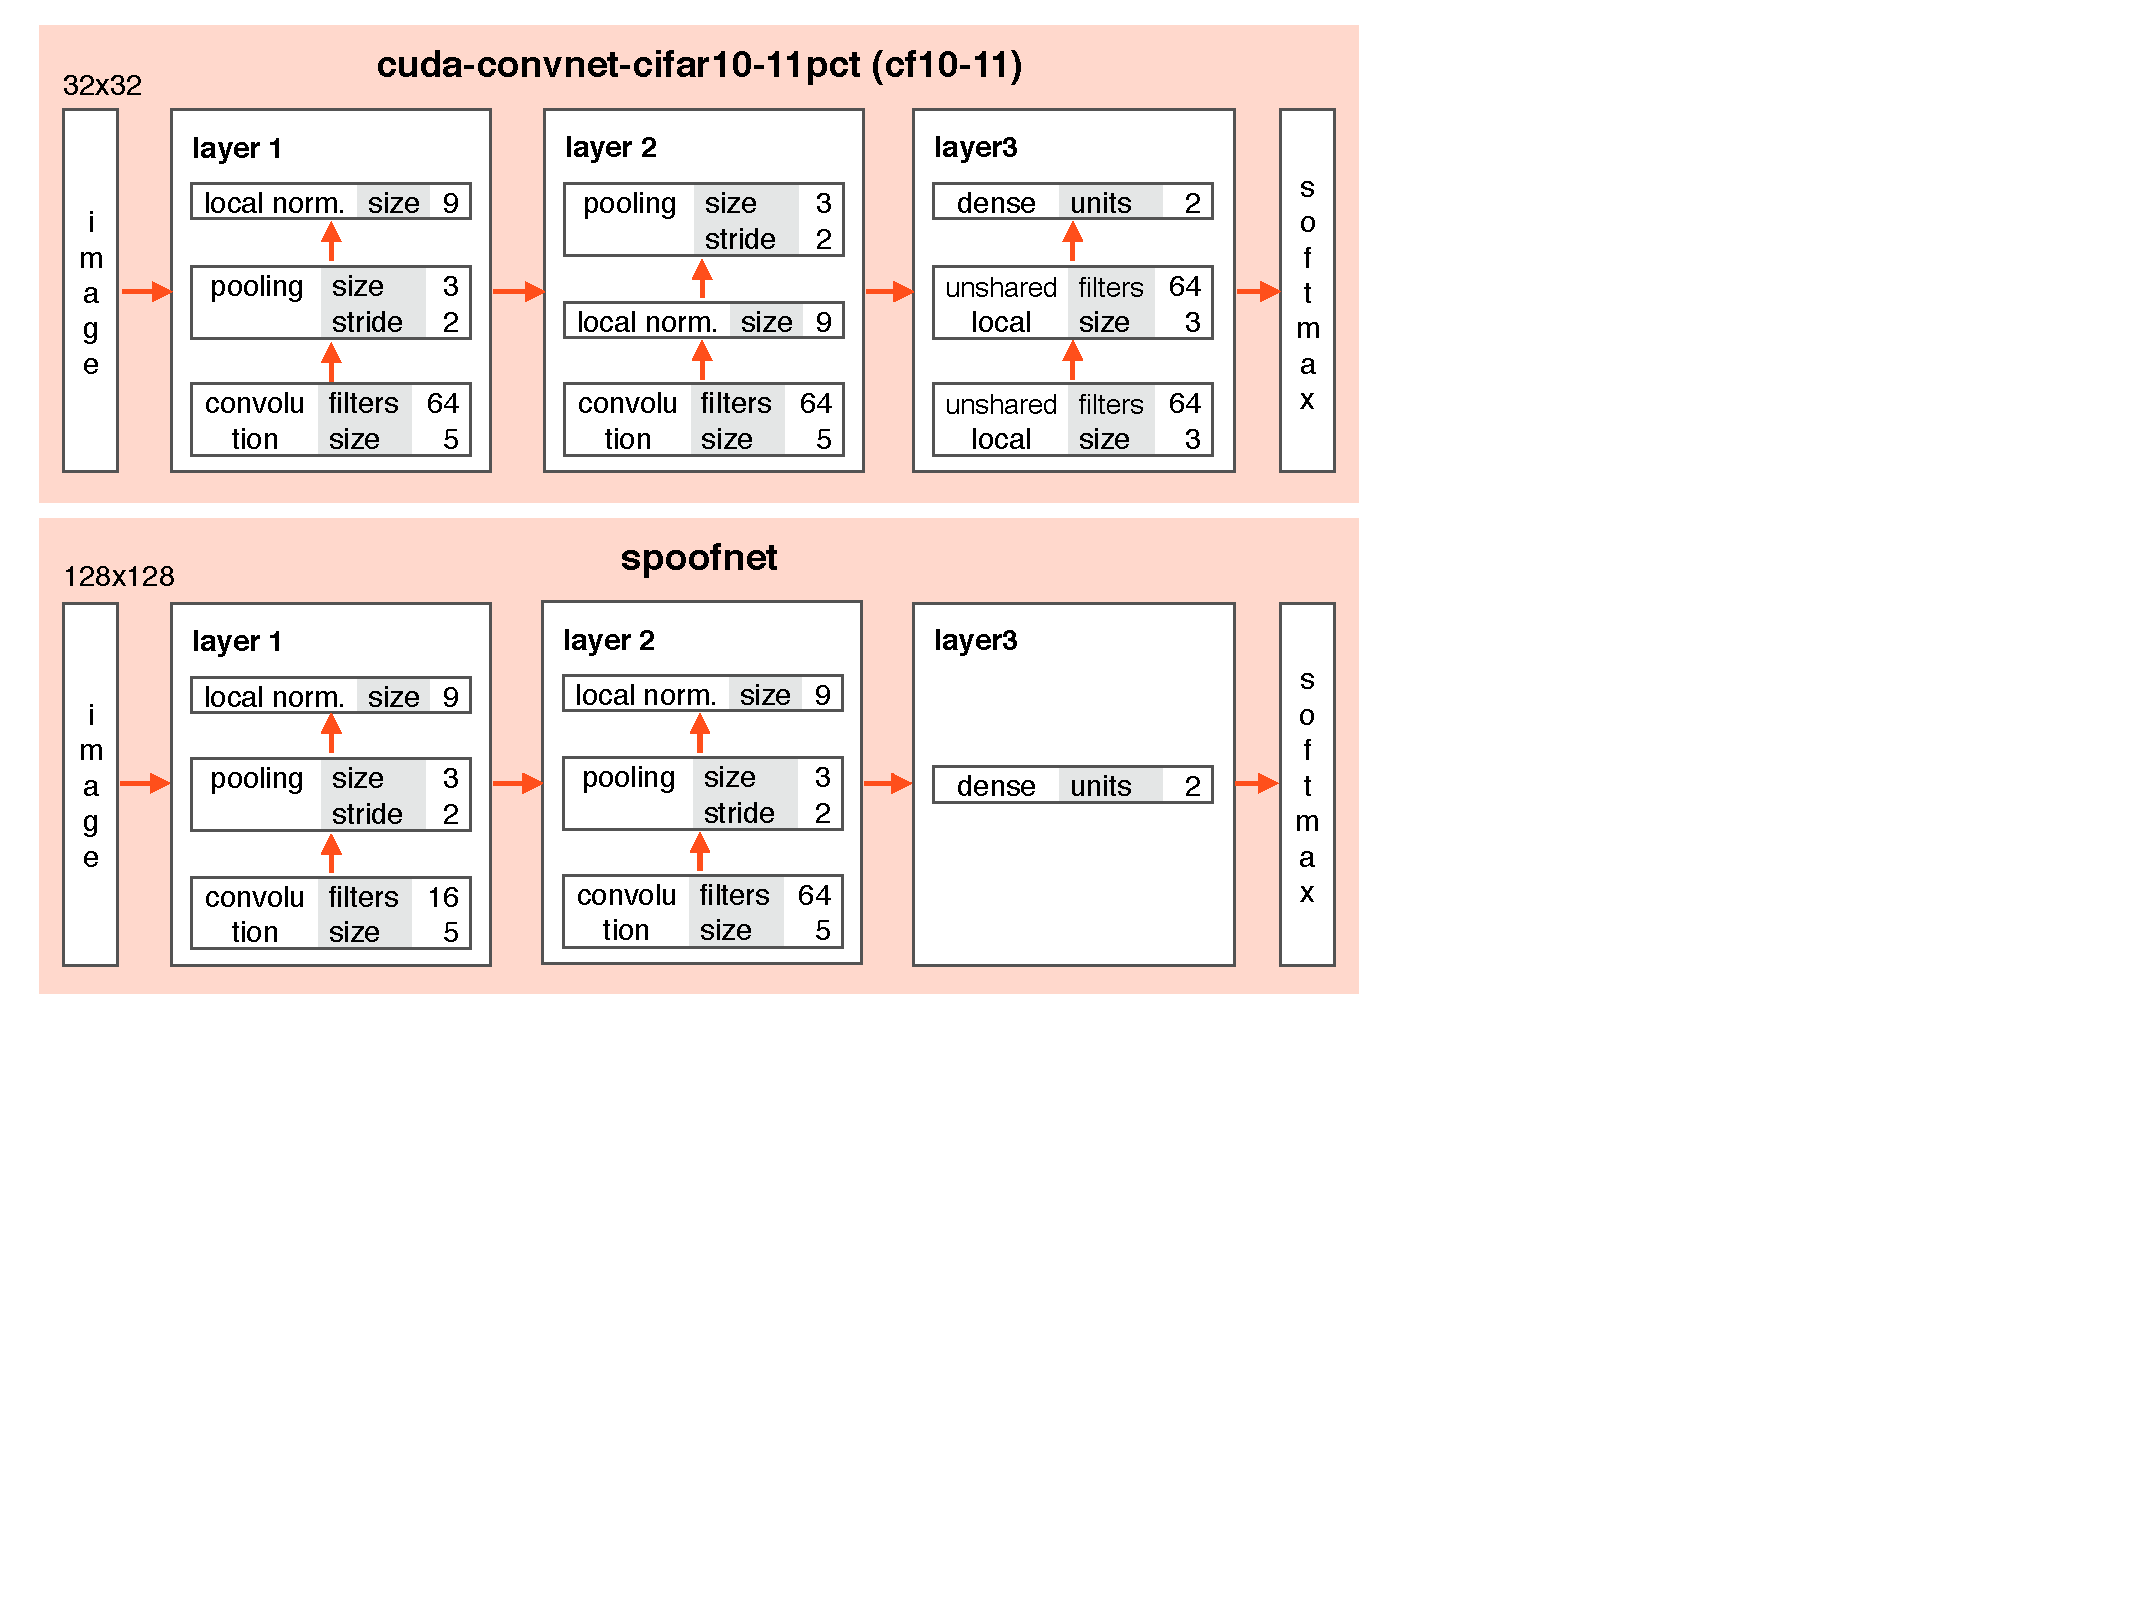
\includegraphics[width=1.0\linewidth]{cuda-convnet.pdf}
\caption{
Architecture of convolutional network found in the Cuda-convnet library~\cite{Krizhevsky:cuda-convnet:2012} and here used as reference for filter optimization (\emph{cf10-11}, top). Proposed network architecture extending upon~\emph{cf10-11} to better suiting spoofing detection problems (\emph{spoofnet}, bottom). Both architectures are typical examples where domain knowledge has been incorporated for increased performance.
}
\label{fig:cudaconvnet}
\end{center}
\end{figure}

We now turn our attention to a different approach for tackling the problem. Instead of optimizing the architecture, we explore the filter weights and how to learn them for better characterizing real and fake samples. Our approach for FO is at the origins of convolutional networks and consists of learning filter weights via the well-known back-propagation algorithm~\cite{LeCun:1998}. Indeed, due to a refined understanding of the optimization process and the availability of plenty of data and processing power, back-propagation has been the gold standard method in deep networks for computer vision in the last years~\cite{Krizhevsky:2012,Simonyan:2014,Zeiler:2014}.

For optimizing filters, we need to have an already defined architecture. We start optimizing filters with a standard public convolutional network and training procedure. This network is available in the Cuda-convnet library~\cite{Krizhevsky:cuda-convnet:2012} and is currently one of the best performing architectures in CIFAR-10,\footnote{\url{http://www.cs.toronto.edu/~kriz/cifar.html}} a popular computer vision benchmark in which such network achieves 11\% of classification error. Hereinafter, we call this network \emph{cuda-convnet-cifar10-11pct}, or simply \emph{cf10-11}.

Fig.~\ref{fig:cudaconvnet} depicts the architecture of \emph{cf10-11} in the top panel and is a typical example where domain knowledge has been incorporated for increased performance. We can see it as a three-layered network in which the first two layers are convolutional, with operations similar to the operations used in architecture optimization (AO). In the third layer, \emph{cf10-11} has two sublayers of unshared local filtering and a final fully-connected sublayer on top of which softmax regression is performed. A detailed explanation of the operations in \emph{cf10-11} can be found in~\cite{Krizhevsky:cuda-convnet:2012}.

In order to train~\emph{cf10-11} in a given benchmark, we split the training images into four batches observing the same balance of real and fake images. After that, we follow a procedure similar to the original\footnote{\url{https://code.google.com/p/cuda-convnet/wiki/Methodology}.} for training~\emph{cf10-11} in all benchmarks, which can be described as follows:

\begin{enumerate}
\item For 100 epochs, train the network with a learning rate of $10^{-3}$ by considering the first three batches for training and the fourth batch for validation;
\item For another 40 epochs, resume training now considering all four batches for training;
\item Reduce the learning rate by a factor of 10, and train the network for another 10 epochs;
\item Reduce the learning rate by another factor of 10, and train the network for another 10 epochs.
\\
\end{enumerate}

% Once~\emph{cf10-11} is trained in a given benchmark, prediction on test samples is performed by softmax 
% The network learned after this process is the one used to evaluate the benchmarks.

After evaluating filter learning on the \emph{cf10-11} architecture, we also wondered how filter learning could benefit from an optimized architecture incorporating domain-knowledge of the problem. Therefore, extending upon the knowledge obtained with AO as well as with training~\emph{cf10-11} in the benchmarks, we derived a new architecture for spoofing detection that we call~\emph{spoofnet}. Fig.~\ref{fig:cudaconvnet} illustrates this architecture in the bottom panel and has three key differences as compared to~\emph{cf10-11}. First, it has 16 filters in the first layer instead of 64. Second, operations in the second layer are stacked in the same order that we used when optimizing architectures (AO). Third, we removed the two unshared local filtering operations in the third layer, as they seem inappropriate in a problem where object structure is irrelevant.

These three modifications considerably dropped the number of weights in the network and this, in turn, allowed us to increase of size of the input images from $32\times32$ to $128\times128$. This is the fourth and last modification in~\emph{spoofnet}, and we believe that it might enable the network to be more sensitive to subtle local patterns in the images.

In order to train~\emph{spoofnet}, the same procedure used to train~\emph{cf10-11} is considered except for the initial learning rate, which is made $10^{-4}$, and for the number of epochs in each step, which is doubled. These modifications were made because of the decreased learning capacity of the network.
% However, given that~\emph{spoofnet} is much faster than~\emph{cf10-11} to process images, the overall training time was not increased.

% For the extended architecture we proposed here, we have developed a slightly different training methodology that the one used for the Krizhevsky \emph{et al.}'s model.
% Indeed, we increase by two the number of training epochs in the three phases described above adding up 320 epochs, since we reduce the number of filter in the first convolutional layer.
% Moreover, we setup the starting learning rate equal to $10^{-4}$, instead of $10^{-3}$ as done in Krizhevsky's methodology.


% We also propose an extended version of Alex's architecture, which can be seen as a reduced one to the complexity of spoofing problem.
% Indeed, we: 1) use only 16 filters in the first convolutional layer; 2) remove the third layer, the locally-connected layer. 
% Moreover $128 \times 128 \times C$ image pixels are used as input for this extended version.
% These modifications made the evaluation time for the extended network at least twice faster.


% The domain knowledge convolution network chosen to be used here for filter learning via backpropagation is the one used in~\cite{Krizhevsky:2012} which achieves accuracy near $90\%$ on CIFAR-10 dataset. 

% In the following we describe in details these architectures, their training methodologies together with the data preparation for and how data augmentation is employed to boost the learning processing.

% More specifically Krizhevsky \emph{et al.}'s (or simply Alex) architecture~\cite{Krizhevsky:2012} can be seen as composed of four layers. 
% In the first one, convolutional operation with 64 filters of $5\times 5$, followed by a $3\times 3$ max-pooling operation with stride 2, and $9 \times 9$ local response/contrast normalization. 
% In the second layer, convolutional operation with 64 filters of $3 \times 3$, followed by $9\times 9$ local response/contrast normalization and then $3\times 3$ max-pooling operation with stride 3.
% In the third layer, we have two locally-connected operations with unshared weight, using 64 and 32 filters of $3\times 3$, respectively.
% The final layer, which can be seen as the classification one, is composed of a fully connected operation to two neurons attached to softmax operations, which can be interpreted as probabilities, where the backpropation starts the learning task with target classes. For such, an objective function should be defined. In this case a (multinomial) logistic regression objective one.
% This network can also be seen as being composed of 11 layers, if each operation is considered as a layer.

% The input for this network uses $32 \times 32 \times c$ image pixels - the standard size of CIFAR-10 dataset, where $c$ stands for the number of channels in the images of each benchmark. 
% But here we adopt $c=1$ for the benchmarks using grayscale images, and keep $c=3$ when color images are available.

Finally, in order to reduce overfitting, data augmentation is used for training both networks according to the procedure of~\cite{Krizhevsky:2012}. For \emph{cf10-11}, five $24\times24$ image patches are cropped out from the $32\times32$ input images. These patches correspond to the four corners and central region of the original image, and their horizontal reflections are also considered. Therefore, ten training samples are generated from a single image. For \emph{spoofnet}, the procedure is the same except for the fact that input images have $128\times128$ pixels and cropped regions are of $112\times112$ pixels. During prediction, just the central region of the test image is considered.


\subsection{Elementary Preprocessing}
\label{sec:preproc}

A few basic preprocessing operations were executed on face and fingerprint images in order to properly learn representations for these benchmarks. 
This preprocessing led to images with sizes as presented in Table~\ref{tab:databases:experiments} and are described in the next two sections.

\begin{table}[tb!]
\begin{center}
\caption{Input image dimensionality after basic preprocessing on face and fingerprint images (highlighted). See Section~\ref{sec:preproc} for details.}
\label{tab:databases:experiments}
\begin{tabular}{clc}
\hline
\multirow{2}{*}{Modality}
& \multirow{2}{*}{Benchmark}
                                             & Dimensions \\
&                                            & $columns \times rows$ \\
\hline
\hline
\multirow{3}{*}{Iris}
&Warsaw~\cite{Czajka:MMAR:2013}              & $640 \times  480$ \\
&Biosec~\cite{Ruiz-Albacete:BIOID:2008}      & $640 \times  480$ \\
&MobBIOfake~\cite{Sequeira:VISAPP:2014:base} & $250 \times  200$ \\
\hline
\multirow{2}{*}{Face}
& Replay-Attack~\cite{Chakka:IJCB:2011}      & $\mathbf{200 \times  200}$ \\
& 3DMAD~\cite{Chingovska:ICB:2013}           & $\mathbf{200 \times  200}$ \\
\hline
\multirow{4}{*}{Fingerprint} 
&Biometrika~\cite{Ghiani:ICB:2013}           & $\mathbf{312 \times  372}$ \\
&CrossMatch~\cite{Ghiani:ICB:2013}           & $\mathbf{480 \times  675}$ \\
&Italdata~\cite{Ghiani:ICB:2013}             & $\mathbf{384 \times  432}$ \\
&Swipe~\cite{Ghiani:ICB:2013}                & $\mathbf{187 \times  962}$ \\
\hline

\end{tabular}
\end{center}
\end{table}

\subsubsection{Face Images}

Given that the face benchmarks considered in this work are video-based, we first evenly subsample 10 frames from each input video. Then, we detect the face position using Viola \& Jones~\cite{Viola:IJCV:2001} and crop a region of $200 \times 200$ pixels centered at the detected window.

\subsubsection{Fingerprint Images}
Given the diverse nature of images captured from different sensors, here the preprocessing is defined according to the sensor type.
\begin{enumerate}[(a)]
\item \emph{Biometrika}: we cropped the central region of size in columns and rows corresponding to 70\% of the original image dimensions. 
\item \emph{Italdata} and \emph{CrossMatch}: we cropped the central region of size in columns and rows respectively corresponding to 60\% and 90\% of the original image columns and rows.
\item \emph{Swipe}: As the images acquired by this sensor contain a variable number of blank rows at the bottom, the average number of non-blank rows $M$ was first calculated from the training images.
Then, in order to obtain images of a common size with non-blank rows, we removed their blank rows at the bottom and rescaled them to $M$ rows. Finally, we cropped the central region corresponding to 90\% of original image columns and $M$ rows.
\end{enumerate}

The rationale for these operations is based on the observation that fingerprint images in LivDet2013 tend to have a large portion of background content and therefore we try to discard such information that could otherwise mislead the representation learning process.
The percentage of cropped columns and rows differs among sensors because they capture images of different sizes with different amounts of background.

For architecture optimization (AO), the decision to use image color information was made according to 10-fold validation (see Section~\ref{sec:ao}), while for filter optimization (FO), color information was considered whenever available for a better approximation with the standard cf10-11 architecture. Finally, images were resized to $32\times32$ or $128\times128$ to be taken as input for the cf10-11 and spoofnet architectures, respectively. 

\subsection{Evaluation Protocol}
\label{sec:evalprot}

For each benchmark, we learn deep representations from their training images according to the methodology described in Section~\ref{sec:ao} for architecture optimization (AO) and in Section~\ref{sec:fo} for filter optimization (FO).
We follow the standard evaluation protocol of all benchmarks and evaluate the methods in terms of detection accuracy (ACC) and half total error rate (HTER), as these are the metrics used to assess progress in the set of benchmarks considered herein. Precisely, for a given benchmark and convolutional network already trained, results are obtained by:

\begin{enumerate}
\item Retrieving prediction scores from the testing samples;
\item Calculating a threshold $\tau$ above which samples are predicted as attacks;
\item Computing ACC and/or HTER using $\tau$ and test predictions.
\end{enumerate}

The way that $\tau$ is calculated differs depending on whether the benchmark has a development set or not (Table~\ref{tab:databases}). Both face benchmarks have such a set and, in this case, we simply obtain $\tau$ from the predictions of the samples in this set. 
Iris and fingerprint benchmarks have no such a set, therefore $\tau$ is calculated depending on whether the convolutional network was learned with AO or FO.

In case of AO, we calculate $\tau$ by joining the predictions obtained from 10-fold validation (see Section~\ref{sec:ao}) in a single set of positive and negative scores, and $\tau$ is computed as the point that lead to an equal error rate (EER) on the score distribution under consideration. 
In case of FO, scores are probabilities and we assume $\tau=0.5$. ACC and HTER are then trivially computed with $\tau$ on the testing set.

It is worth noting that the Warsaw iris benchmark provides a supplementary testing set that here we merge with the original testing set in order to replicate the protocol of~\cite{LivDet:Iris:2013}.
Moreover, given face benchmarks are video-based and that in our methodology we treat them as images (Section~\ref{sec:preproc}),
we perform a score-level fusion of the samples from the same video according to the max rule~\cite{Ross:HM:2006}. This fusion is done before calculating $\tau$.


\subsection{Implementation}
\label{sec:implementationdetais}

Our implementation for architecture optimization (AO) is based on Hyperopt-convnet~\cite{Bergstra:2013b} which in turn is based on Theano~\cite{Bergstra:SCIPY:2010}.
LibSVM~\cite{Chang:2011} is used for learning the linear classifiers via Scikit-learn.\footnote{http://scikit-learn.org}
The code for feature extraction runs on GPUs due to Theano and the remaining part is multithreaded and runs on CPUs.
We extended Hyperopt-convnet in order to consider the operations and hyperparameters as described in Appendix~\ref{sec:convnet_ops} and Section~\ref{sec:ao} and we will make the source code freely available in~\cite{Chiachia:2014b}.
Running times are reported with this software stack and are computed in an Intel i7 @3.5GHz with a Tesla K40 that, on average, takes less than one day to optimize an architecture --- i.e., to probe 2,000 candidate architectures --- for a given benchmark.

As for filter optimization (FO), Cuda-convnet~\cite{Krizhevsky:cuda-convnet:2012} is used. This library has an extremely efficient implementation to train convolutional networks via back-propagation on NVIDIA GPUs. 
Moreover, it provides us with the cf10-11 convolutional architecture taken in this work as reference for FO.
